% ju 28-Mai-22
\documentclass[a4paper,12pt,fleqn,parskip=half]{scrartcl}
\usepackage[ngerman]{babel}
\usepackage[utf8]{inputenc}
\usepackage[T1]{fontenc}

% Schrift
%\usepackage{lmodern}
\usepackage[osf,sc]{mathpazo} 
\usepackage[scale=.9,semibold]{sourcecodepro}   
\usepackage[osf]{sourcesanspro}  

\usepackage[headsepline]{scrlayer-scrpage}
\pagestyle{scrheadings}
\clearpairofpagestyles

\usepackage[table,dvipsnames,usenames]{xcolor}
\usepackage{textcase}
\usepackage{nameref}
\usepackage{hyperref}
\usepackage{tabularx}
\usepackage{multirow}
\usepackage{multicol}
\usepackage{caption, booktabs}
\usepackage{graphicx} 
\usepackage{scrhack}    
\usepackage{url}%% Links
\usepackage[inline]{enumitem}
\usepackage{pifont}
\usepackage{eurosym}% \euro 20,-
\usepackage{amsmath}
\usepackage{amsfonts}
\usepackage{amssymb}
\usepackage{array}            % Extending the array and tabular environments
\usepackage{chngcntr}         % Change the resetting of counters
\usepackage[version=4]{mhchem}
\usepackage{stmaryrd}
\usepackage{siunitx}
\usepackage{float}
\usepackage{csquotes}
\usepackage{subcaption}
\usepackage{mathtools}
\usepackage{icomma}%Dezimaltrennzeichen
\usepackage{multimedia}%Video: \movie[externalviewer]{(video.mov)}{video.mov}
\usepackage{epstopdf}
\usepackage{footnote}
\usepackage{qrcode}% Anwendung: \qrcode[hyperlink,level=Q,version=2,height=1cm]{\website}
\usepackage{underscore}% Unterstrich ____

% PDF Dokumente einbinden
\usepackage{pdfpages}% \includepdf[pages=-]{Tabellen/Excel.pdf}
\RequirePackage{lastpage}  % Pagecounter

\addto\captionsngerman{%
\renewcommand{\figurename}{Abb.}
\renewcommand{\tablename}{Tab.}
}

% listings
\usepackage{listings}
\lstset{basicstyle=\linespread{1}\ttfamily\small,floatplacement=!htb,captionpos=t,abovecaptionskip=.5\baselineskip,belowcaptionskip=.5\baselineskip,upquote=true,showstringspaces=false,inputencoding=utf8,tabsize=4,
    	keywordstyle=\bfseries ,
	commentstyle=\color{rot5},
	stringstyle=\color{orange},
	breaklines=true,
  	postbreak=\mbox{\textcolor{black}{$\hookrightarrow$}\space},
	breakatwhitespace=false
}
\lstset{literate={á}{{\'a}}1 {é}{{\'e}}1 {í}{{\'i}}1 {ó}{{\'o}}1 {ú}{{\'u}}1 {Á}{{\'A}}1 {É}{{\'E}}1 {Í}{{\'I}}1 {Ó}{{\'O}}1 {Ú}{{\'U}}1 {à}{{\`a}}1 {è}{{\`e}}1 {ì}{{\`i}}1 {ò}{{\`o}}1 {ù}{{\`u}}1 {À}{{\`A}}1 {È}{{\'E}}1 {Ì}{{\`I}}1 {Ò}{{\`O}}1 {Ù}{{\`U}}1 {ä}{{\"a}}1 {ë}{{\"e}}1 {ï}{{\"i}}1 {ö}{{\"o}}1 {ü}{{\"u}}1 {Ä}{{\"A}}1 {Ë}{{\"E}}1 {Ï}{{\"I}}1 {Ö}{{\"O}}1 {Ü}{{\"U}}1 {â}{{\^a}}1 {ê}{{\^e}}1 {î}{{\^i}}1 {ô}{{\^o}}1 {û}{{\^u}}1 {Â}{{\^A}}1 {Ê}{{\^E}}1 {Î}{{\^I}}1 {Ô}{{\^O}}1 {Û}{{\^U}}1 {œ}{{\oe}}1 {Œ}{{\OE}}1 {æ}{{\ae}}1 {Æ}{{\AE}}1 {ß}{{\ss}}1 {ű}{{\H{u}}}1 {Ű}{{\H{U}}}1 {ő}{{\H{o}}}1 {Ő}{{\H{O}}}1 {ç}{{\c c}}1 {Ç}{{\c C}}1 {ø}{{\o}}1 {å}{{\r a}}1 {Å}{{\r A}}1 {€}{{\EUR}}1 {£}{{\pounds}}1 {~}{{\textasciitilde}}1 {-}{{-}}1 }

% bibliography
\usepackage[
    bibencoding=utf8,
    backend=biber,% bibtex, biber
    backref=false,backrefstyle=three+,url=true,urldate=comp,abbreviate=false,maxnames=20
]{biblatex} %Paket laden
\DeclareBibliographyCategory{cited}
\let\defaultcite\cite\renewcommand*\cite[2][]{\addtocategory{cited}{#2}\defaultcite[#1]{#2}}
\let\defaulttextcite\textcite\renewcommand*\textcite[2][]{\addtocategory{cited}{#2}\defaulttextcite[#1]{#2}}
\setcounter{biburllcpenalty}{7000}
\setcounter{biburlucpenalty}{8000}
\AfterPackage{biblatex}{
	\PreventPackageFromLoading[\errmessage{Sie haben versucht, das Cite-Paket zu laden, das nicht mit biblatex kompatibel ist.}]{cite}
}

\hypersetup{%
	%pdftitle={\titel},
	%pdfsubject={Latex},
	%pdfauthor={\autor},
	%pdfcreator={\autor}, 
	bookmarksnumbered=true,
	breaklinks=true,
	%colorlinks=true,	   
	linkcolor=rot5,		
	filecolor=blau5,		
	urlcolor=blau5,			
	citecolor=ForestGreen
}

\linespread{1.1}
\setlist{itemsep=0pt}
\widowpenalty10000
\clubpenalty10000
\tolerance1000   

\usepackage[left=2cm,right=2cm,top=1cm,bottom=1cm,includeheadfoot]{geometry}
%\usepackage[left=4cm,right=2cm,top=1cm, bottom=1cm,includeheadfoot]{geometry}
%\usepackage[left=6cm,right=1cm,top=1cm, bottom=1cm,includeheadfoot]{geometry}
%\usepackage[landscape=true,left=2cm,right=2cm,top=1cm,bottom=1cm,includeheadfoot]{geometry}%quer

% eigene Farbe definieren
% Adobe Prozessfarben: CMYK: 100,50,0,35 -> 1,0.5,0,0.35
\definecolor{orange}{cmyk}{0,0.55,0.61,0}   % 0,55,61,0
\definecolor{blau5}{cmyk}{1,0.77,0.1,0.01}  % 100,77,10,
\definecolor{rot5}{cmyk}{0.22,1,1,0.19}     % 22,100,100,19
\definecolor{grau2}{cmyk}{0,0,0,0.1}        % 0,0,0,40
\definecolor{blau}{cmyk}{0.93,0.66,0,0.21}% 

% Literatur
\bibliography{content/literatur}
\bibliography{content/literatur-kfz}
\bibliography{content/literatur-sport}

%%%%%%%%%%%%%%%%%%%%%%%%%%%%%%%%%%%%%%%%%%%%%%%%%%%%%%%
\newcommand{\name}{Jan Unger}% anpassen!!!!!
\newcommand{\thema}{02-Verbrennungsmotor-Elektrik}
\newcommand{\quelle}{\name}
\newcommand{\website}{https://bw-ju.de/}
\newcommand{\github}{https://github.com/ju1-eu}
%%%%%%%%%%%%%%%%%%%%%%%%%%%%%%%%%%%%%%%%%%%%%%%%%%%%%%%

\ihead{\textbf{Quelle:} \quelle}%{Kopfzeile innen}
\ohead{\textbf{Datum:} \today}  %{Kopfzeile außen}

\ifoot{\textbf{Thema:} \thema}  %{Fußzeile  innen}
\ofoot{Seite {\thepage} von {\pageref{LastPage}}}%{Fußzeile  außen}

\title{\thema}
\author{\name}
\date{\today}

\begin{document}
	%\thispagestyle{empty}
	%\maketitle
	%\newpage
	%\setcounter{page}{1}

	%%%%%%%%%%%%%%%%%%%%%%%%%%%%%%%%%%%%%%%%%%%
	\begin{center}
		\textbf{\Large \thema}%14pt
		\vspace{0.8em}
		
		%\datum	
		%\qrcode[hyperlink,level=Q,version=2,height=1cm]{\website}
		\qrcode[hyperlink,level=Q,version=2,height=1cm]{\github}
	\end{center}
	%%%%%%%%%%%%%%%%%%%%%%%%%%%%%%%%%%%%%%%%%%%

	\subsection*{Keywords}%\label{sec:Deadline}\index{Deadline}
	% Checkliste
	\begin{itemize}[label=\checkmark] %\itemsep -2pt
		\item Begriff 
	\end{itemize}

    %%%%%%%%%%%%%%%%%%%%%%%%%%%%%%%%%%%%%%%%%%%%%%%%%%%%%%%%%%%%%%%%%%

	% anpassen
	%\input{content/tex/neu}
	%ju 28-Mai-22 02-Verbrennungsmotor-Elektrik.tex
\section{Kraftstoffpumpenrelais}\label{kraftstoffpumpenrelais}

\textbf{Nenne 3 Abschaltmöglichkeiten. Weshalb werden überhaupt das
Kraftstoffpumpenrelais und damit die Kraftstoffförderpumpe
abgeschaltet?}

\begin{enumerate}
\item
  \textbf{Konventionelle Abschaltung durch das Steuergerät}

  Bei Abstellung des Motors wird das Kraftstoffförderpumpenrelais vom SG
  nicht mehr angesteuert, somit wird kein Kraftstoff mehr gefördert.
\item
  \textbf{Ausfall des Bezugsmarken-Drehzahlgebers}

  Fällt der \emph{Bezugsmarken-Drehzahlgeber} aus, während des Betriebs
  oder bei Stillstand des Motors, kann das SG den ersten Zylinder nicht
  mehr zuordnen. Der Motor springt nicht mehr an. Ist dieses der Fall,
  schaltet das SG das Kraftstoffförderpumpenrelais ab. Mit dem
  Abschalten werden nachfolgende Komponenten nicht mehr mit Spannung
  versorgt:

  \begin{itemize}
  \item
    Kraftstoffförderpumpe
  \item
    alle Einspritzventile
  \item
    Tankentlüftungsventil
  \item
    Lambdasondenheizung
  \end{itemize}
\item
  \textbf{Volllaufsicherung}

  Sollte der Motor durch ein unbeabsichtigtes Manöver des Fahrers einmal
  zum Stillstand gekommen sein, liefert der
  \emph{Bezugsmarken-Drehzahlgeber} kein Signal mehr, aufgrund des
  stehenden Motors, an das SG. Sobald dieses Signal ausbleibt, schaltet
  das SG das Kraftstoffpumpenrelais ab, die Kraftstoffförderpumpe
  fördert keinen Kraftstoff mehr.

  \textbf{Hintergrund}: Es kann ja sein, dass ein Einspritzventil
  undicht ist, das Einlassventil offen steht, somit würde, wenn die
  Kraftstoffförderpumpe weiterhin Kraftstoff fördert, in den
  entsprechenden Zylinder Kraftstoff eingespritzt. Er läuft also voll.
  Wird nun, nach einer Weile, wieder ein Startvorgang durchgeführt,
  kommt es zu einem kapitalen Folgeschaden, da nach dem
  \emph{Pascalschen Gesetz}, Flüssigkeiten sich nicht zusammendrücken
  lassen. Die Folge wären mechanische Defekte am Kurbeltrieb und Kolben.
\end{enumerate}

\textbf{Verunfallen}

Kommt es zu einem Unfall, mit dem Auslösen des Airbags und
anschließenden Überschlägen des Fahrzeugs, möchte man nicht, dass die
Kraftstoffförderpumpe weiterhin Kraftstoff fördert. Es ist auch möglich,
dass aus einer Kraftstoffleitung unkontrolliert Kraftstoff austritt, der
sich unweigerlich an heißen Fahrzeugteilen, oder an
Kurzschlussfunkenbildung entzünden würde.

\textbf{Wann läuft die Kraftstoffpumpe an?} $\to$ über
Türkontaktschalter

\section{Sekundärluftpumpe}\label{sekundaerluftpumpe}

Das \textbf{Sekundärluftsystem} wird bei Ottomotoren in der
Kaltstartphase (3-5 Min.) aktiviert, um die Abgasbestandteile HC und CO
in der Warmlaufphase zu minimieren, durch eine thermische
Nachverbrennung.

\textbf{Sekundärluftpumpe} Umgebungsluft anzusaugen und diese in den
Abgaskrümmer hinter den Auslassventilen einzublasen.

Durch Oxidation entsteht Wärme (unverbrannte Kohlenwasserstoffe
reagieren mit Sauerstoff, Wärmeenergie wird frei)

\emph{Ziel} 350 °C >>light-off-Point<< schnell erreichen.)

\emph{Betriebstemperatur Katalysator} 650 bis 800 °C

\section{3-Wege-Kat}\label{wege-kat}

\textbf{Welche Schadstoffe werden im Oxidationskatalysator zu welchen
Stoffen umgewandelt?}

\textbf{Aufbau Katalysator} Keramik- o. Metallträger, Zwischenschicht
(Wash-Coat, Oberfläche vergrößern), katalytisch aktive Schicht
(Edelmetalle: Rhodium, Platin)

\emph{Die chemischen Reaktionsgleichungen lauten:}

\begin{enumerate}
\item
  \textbf{Kohlenmonoxid} $CO$ + $O_2$ wird umgewandelt zu $CO_2$ =
  Kohlendioxid, Sauerstoff wird verbraucht

  \begin{itemize}
  \item
    Katalysator = Platin $\to$ Oxidationsprozess
  \end{itemize}
\item
  \textbf{unverbrannte Kohlenwasserstoffe} $HC$ + $O_2$ werden
  umgewandelt zu $CO_2$ + $H_2O$ = Kohlendioxid und Wasser,
  Sauerstoff wird verbraucht

  \begin{itemize}
  \item
    Katalysator = Platin $\to$ Oxidationsprozess
  \end{itemize}
\item
  \textbf{Stickoxide} $NO_\text{x}$ wird umgewandelt zu $N_2$ +
  $O_2$, Sauerstoff wird freigesetzt

  \begin{itemize}
  \item
    Katalysator = Rhodium $\to$ Reduktionsprozess
  \end{itemize}
\end{enumerate}

\textbf{Weshalb werden Oxidationskatalysatoren vor den Partikelfiltern
eingebaut?}

Durch den Oxidationsprozess entsteht eine höhere Abgastemperatur, diese
höhere Abgastemperatur unterstützt die Regenration des Partikelfilters,
das heißt, die Partikel können dadurch abgebrannt werden.

\section{AdBlue}\label{adblue}

\textbf{Was ist an dem Motor anders? Warum braucht der Motor AdBlue?}

\begin{itemize}
\item
  höheres Verdichtungsverhältnis $\to$ weniger Kraftstoff notwendig
\item
  höhere Wärme und Druck
\item
  mehr Stickoxide
\end{itemize}

AdBlue

\begin{itemize}
\item
  Reduktionsmittel
\item
  gefriert - 11 °C
\item
  32,5 \% ca. 1/3 Harnstoff + 2/3 demineralisiertes Wasser (rein)
\end{itemize}

\textbf{chemische Prozess AdBlue} Hydrolysestrecke Harnstoff $\to$
Ammoniak (säurehaltig) $\to$ SCR-Kat $\to$ $NO_\text{x}$ +
Ammoniak umgewandelt in Stickstoff + Wasser

\section{Wie kann ich den Einsatz von Kraftstoff reduzieren?
(Nacheinspritzung
weglassen)}\label{wie-kann-ich-den-einsatz-von-kraftstoff-reduzieren-nacheinspritzung-weglassen}

$\to$ Ausgangspunkt: Temperatur 550 °C notwendig

\textbf{Wie?}

\begin{itemize}
\item
  höherer Druck $\to$ höhere Temperatur
\item
  Ansauglufterwärmung (Kondensationsverluste reduzieren)
\item
  Glühkerzen

  \begin{itemize}
  \item
    \emph{Vorglühen} (Kaltstart)
  \item
    \emph{Zwischen glühen} (weniger Kraftstoff einsetzen)
  \end{itemize}
\end{itemize}

\section{Schubabschaltung
(Voraussetzung)}\label{schubabschaltung-voraussetzung}

\begin{enumerate}
\item
  Drosselklappen geschlossen (Leerlaufkontakt)
\item
  Kein Kraftstoff eingespritzt
\item
  Motortemperatur $>$ 80 °C
\item
  Drehzahl $>$ wieder Einsetzdrehzahl (1400-1700 U/min)
\end{enumerate}

\section{Schichtladebetrieb - homogene
Gemischbildung}\label{schichtladebetrieb-homogene-gemischbildung}

\textbf{Umschalten} erfolgt durch Gas geben: Schichtladebetrieb $\to$
homogene Gemischbildung

\textbf{Wie kann ich das klingeln vermeiden?}

$\to$ Ausgangslage Verdichtungsverhältnis bleibt konstant

$\to$ Brennraumtemperatur herabsetzen, wie?

\begin{enumerate}
\item
  \textbf{Zündzeitpunkt auf Spät verstellen,} d.h. 15° vor OT

  \begin{itemize}
  \item
    $\to$ Verbrennungshöchstdruck wird später erreicht, 20° nach OT
  \item
    Kolben wird weiter geschoben durch die vorhergehende Verbrennung
  \item
    AV öffnet 148° nach OT, wir haben ein heißeres Abgas

    \begin{itemize}
    \item
      $\to$ der Katalysator kommt schneller auf Betriebstemperatur
    \item
      Wenn der Raum größer wird, nimmt der Druck ab und damit die
      Temperatur. (Hier nicht voll ausgenutzt, und damit habe ich ein
      heißeres Abgas)
    \end{itemize}
  \item
    \textbf{weniger Leistung} wird in Kauf genommen
  \end{itemize}
\item
  \textbf{Kraftstoff Einspritzen}

  durch den Kraftstoff Einspitzen entziehe ich dem Verbrennungsprozess
  Wärme, dadurch wird die Brennraumtemperatur geringer, geringerer Druck
  und dadurch die Neigung zum Klingeln beseitigt
\end{enumerate}

\textbf{Wärmekraftmaschine}

Ottomotor / \textbf{Gleichraumverbrennung} / Kraftstoff-Luft Gemisch
verdichten reicht nicht aus um einen sehr hohen Verbrennungsdruck und
Temperatur zu bekommen, hier ist eine Zündkerze notwendig.

Vor Ende des Verdichtungstaktes 25-30° vor OT wird das komprimierte
Kraftstoff-Luftgemisch fremdgezündet über den Funken der Zündkerze.
(Entflammung)

Der Verbrennungshöchstdruck wird erreicht bei 3-6° nach OT, damit
bekommt der Kolben ein auf den Deckel und geht nach unten.

\textbf{Höheres Verdichtungsverhältnis} (Nachteil) höhere Drücke $\to$
Kurbelwellenlager

\section{Lenkrollradius}\label{lenkrollradius}

\textbf{Fahrzeug mit Lenkrollradius Null bekommen in der Regel eine
Lenkunterstützung eingebaut? (Hintergrund)}

Lenkrollradius = Lenkrollhalbmesser

\begin{figure}[!ht]% hier: !ht
\centering
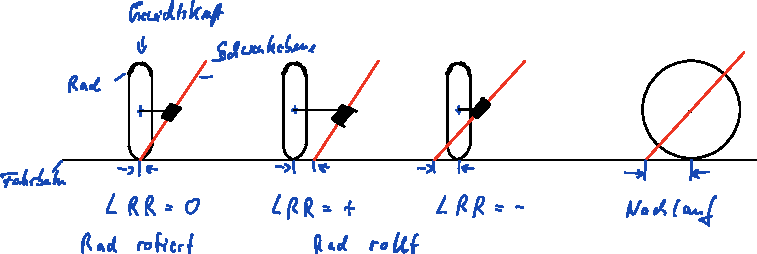
\includegraphics[width=0.6\textwidth]{images/Skizze/27_FT_Lenkrollradius_Nachlauf.pdf}
\caption{Lenkrollradius und Nachlauf}
%\label{fig:}%% anpassen
\end{figure}

Bei einem \textbf{Lenkrollhalbmesser} $0$ trifft die Verlängerung der
Lenkachse (Schwenkachse) mit der Mitte des Radaufstandspunktes in einem
Punkt auf die Fahrbahn.

Erfordert \textbf{hohe Lenkkräfte} im Stand, Rad radiert auf der Stelle,
Vorteil spurstabil.

Lenkrollhalbmesser wird bestimmt durch Sturz, Spreizung und
Einpresstiefe der Felge.

\textbf{Negativer Lenkrollhalbmesser} wird bevorzugt

\begin{itemize}
\item
  Vorteil Fahrzeug bleibt stabilisierend
\item
  Flatterneigung
\item
  Rad rollt um den Drehpunkt herum
\end{itemize}

Nachlauf (Teewagenprinzip)


	%%%%%%%%%%%%%%%%%%%%%%%%%%%%%%%%%%%%%%%%%%%%%%%%%%%%%%%%%%%%%%%%%%
    % Bibliographie
    \printbibliography
\end{document}
